\chapter{受約束系統與哈密頓運動}

\lectureoverview{兩個受約束系統展現了拉格朗日力學為何如此有效：選定適當座標後，無須明確計算約束力，就能寫出運動方程及其守恆律。同樣的例子接著引出哈密頓力學：座標與動量構成相空間，諧振子化為剛性旋轉，而哈密頓的兩個一階方程則取代每個二階的尤拉--拉格朗日方程。}

\section{求解力學問題的意義}

拉格朗日方法的直接目的在於實用。楔塊在地面上滑動、雙擺運動，兩者都能用牛頓定律處理，但未知的接觸力與張力很快就會讓計算變得繁瑣。掌握拉格朗日力學的規則後，同樣的問題便能化為一連串有條理的步驟：
\begin{enumerate}
  \item 選取能標示瞬時位形的獨立座標；
  \item 用這些座標表示動能與勢能；
  \item 構造\(L=T-V\)，並套用尤拉--拉格朗日方程。
\end{enumerate}

就此處的目的而言，只要正確寫出運動方程，問題就算已經\emph{解決}。或許還想求出閉合形式的軌跡，但那是另一回事。力學設定完成後，非線性微分方程可以用數值方法積分。困難之處往往不在積分，而在於找出能納入約束、又不引進冗餘未知力的變數。

\section{在移動的楔塊上滑動的質點}

考慮一個質量為\(M\)的楔塊，受約束而無摩擦地沿水平面滑動。另一個質量為\(m\)的質點則受約束，沿著斜面移動。這個系統有兩個自由度：一個表示楔塊的位置，另一個表示質點在楔塊上的位置。

令
\begin{equation}
  \begin{aligned}
    X&=\text{horizontal position of the wedge corner},\\
    x&=\text{horizontal displacement of the particle}\\[-0.2em]
     &\phantom{={}}\text{from that corner}.
  \end{aligned}
  \label{eq:l6-wedge-coordinates}
\end{equation}
因此，質點的絕對水平座標為\(X+x\)。座標的選法並不唯一；也可以改用沿斜面的距離，或質點的絕對水平座標。只要一組座標不冗餘，且能標示相同的位形，就是合法的選擇；不過，有些選法比其他選法更能清楚呈現系統的結構。

斜面角\(\beta\)固定時，垂直位移\(y\)不是獨立座標：
\begin{equation}
  y=x\tan\beta,
  \qquad
  \dot y=\dot x\tan\beta.
  \label{eq:l6-wedge-constraint}
\end{equation}
我們特別取\(\beta=45^\circ\)，因此\(y=x\)，且
\(\dot y=\dot x\)。這項簡化省去了三角函數因子，但不影響這個例子的要旨。

\begin{figure}[htbp]
  \centering
  \includegraphics[width=0.84\textwidth]{lecture_06_figure_06.png}
  \caption{移動的楔塊、受約束的質點，以及\(45^\circ\)例子中使用的水平與垂直速度分量。}
  \lectureframe{00:10:25}
\end{figure}

楔塊的動能為
\begin{equation}
  T_{M}=\frac{M}{2}\dot X^2.
  \label{eq:l6-wedge-kinetic}
\end{equation}
質點的水平速度為\(\dot X+\dot x\)，垂直速度則為\(\dot x\)。因此，質點的動能為
\begin{equation}
  T_m=\frac{m}{2}\left[(\dot X+\dot x)^2+\dot x^2\right].
  \label{eq:l6-particle-kinetic}
\end{equation}
以\(x=0\)為重力位能的零點，則\(V=mgx\)。所以
\begin{equation}
  L=\frac{M}{2}\dot X^2
    +\frac{m}{2}\left[(\dot X+\dot x)^2+\dot x^2\right]
    -mgx.
  \label{eq:l6-wedge-lagrangian}
\end{equation}

\begin{figure}[htbp]
  \centering
  \includegraphics[width=0.86\textwidth]{lecture_06_figure_07.png}
  \caption{楔塊的幾何、\(V=mgx\)，以及彙整在黑板上的兩項動能。}
  \lectureframe{00:14:15}
\end{figure}

\subsection{正則動量由拉格朗日量定義}

正則動量是由拉格朗日量定義的，不能只憑單一質點的速度來猜：
\begin{align}
  p_X&=\frac{\partial L}{\partial\dot X}
      =M\dot X+m(\dot X+\dot x),
      \label{eq:l6-wedge-pX}\\
  p_x&=\frac{\partial L}{\partial\dot x}
      =m(\dot X+\dot x)+m\dot x.
      \label{eq:l6-wedge-px}
\end{align}
第一個表式就是一般所說的總水平動量：楔塊貢獻\(M\dot X\)，質點貢獻\(m(\dot X+\dot x)\)。在此，它是與座標\(X\)共軛的動量。

\begin{figure}[htbp]
  \centering
  \includegraphics[width=0.86\textwidth]{lecture_06_figure_08.png}
  \caption{分別與楔塊座標\(X\)及質點相對座標\(x\)共軛的正則動量。}
  \lectureframe{00:18:05}
\end{figure}

拉格朗日量沒有明確依賴\(X\)。整個裝置的水平平移變換為
\begin{equation}
  \delta X=\epsilon,
  \qquad
  \delta x=0.
  \label{eq:l6-wedge-translation}
\end{equation}
因此，套用一般的無窮小對稱性規則
\begin{equation}
  \delta q_i=\epsilon f_i(q),
  \qquad
  Q=\sum_i p_i f_i
  \label{eq:l6-noether-rule}
\end{equation}
可得\(Q=p_X\)。換言之，\(X\)是循環座標，而且
\begin{equation}
  \dot p_X=\frac{\partial L}{\partial X}=0.
  \label{eq:l6-wedge-conservation}
\end{equation}

系統沒有相應的垂直平移對稱性。楔塊不能垂直移動，而改變質點的高度會改變重力位能。因此，水平動量守恆；這個受約束子系統的垂直動量則不守恆。

對相對座標而言，尤拉--拉格朗日方程為
\begin{equation}
  \dot p_x=\frac{\partial L}{\partial x}=-mg.
  \label{eq:l6-wedge-force}
\end{equation}
黑板上的這一行曾修正過符號。可靠的推導方式是從\(L=T-V\)出發：由於\(V=mgx\)，拉格朗日量對該座標的導數為\(-mg\)。\(x\)雖然是以水平位移引入的，重力仍會出現在它的方程中，因為約束將這個水平位移與垂直高度\(y=x\)連結起來。

這裡沒有出現法向力或反作用力。這些力會自動取適當的值，以維持約束。牛頓方法會把它們列入，並與加速度一併求解；使用廣義座標便不必處理這些力。

\section{雙擺與座標的巧妙選擇}

現在將兩個單位質量懸掛在兩根無質量、長度為一的桿上。第一根桿與鉛直向下方向的夾角為\(\theta\)。第二個自由度有兩種選擇：使用第二個絕對角\(\phi\)，或使用兩根桿之間的相對角\(\alpha\)。

相對角是較能揭示系統特性的選擇。暫時關閉重力。整個裝置的剛性旋轉會改變絕對取向，卻不改變兩根桿的夾角：
\begin{equation}
  \theta\longrightarrow\theta+\epsilon,
  \qquad
  \alpha\longrightarrow\alpha.
  \label{eq:l6-double-rotation}
\end{equation}
採用這種座標選擇後，旋轉對稱變換只作用在一個座標上。這不表示其他座標系有誤；這樣選只是讓對稱性，以及由此而來的守恆量，更容易看出。

\begin{figure}[htbp]
  \centering
  \includegraphics[width=0.76\textwidth]{lecture_06_figure_09.png}
  \caption{雙擺以\(\theta\)表示第一個絕對角，並以\(\alpha\)表示第二根桿相對於第一根桿的角度。}
  \lectureframe{00:29:20}
\end{figure}

為了求出動能，可以暫時用笛卡兒座標輔助計算。令垂直座標向下為正，第一個擺錘的位置為
\begin{equation}
  x_1=\sin\theta,
  \qquad
  y_1=\cos\theta,
  \label{eq:l6-bob-one-position}
\end{equation}
因此
\begin{equation}
  \dot x_1=\dot\theta\cos\theta,
  \qquad
  \dot y_1=-\dot\theta\sin\theta,
  \qquad
  \dot x_1^2+\dot y_1^2=\dot\theta^2.
  \label{eq:l6-bob-one-velocity}
\end{equation}
第二個擺錘的位置為
\begin{align}
  x_2&=\sin\theta+\sin(\theta+\alpha),\\
  y_2&=\cos\theta+\cos(\theta+\alpha),
  \label{eq:l6-bob-two-position}
\end{align}
例如，
\begin{equation}
  \dot x_2=\dot\theta\cos\theta
  +(\dot\theta+\dot\alpha)\cos(\theta+\alpha),
  \label{eq:l6-bob-two-xvelocity}
\end{equation}
而\(\dot y_2\)也有類似的表式。

\begin{figure}[htbp]
  \centering
  \includegraphics[width=0.88\textwidth]{lecture_06_figure_10.png}
  \caption{兩個擺錘的輔助笛卡兒座標。這些座標用來計算速度，並未作為額外自由度引入。}
  \lectureframe{00:35:25}
\end{figure}

將兩個動能相加，可得下列結果。交叉項來自
\begin{equation*}
  \cos A\cos B+\sin A\sin B=\cos(A-B).
\end{equation*}
\begin{equation}
  T=\dot\theta^2
    +\frac12(\dot\theta+\dot\alpha)^2
    +\dot\theta(\dot\theta+\dot\alpha)\cos\alpha.
  \label{eq:l6-double-kinetic}
\end{equation}

\begin{classroomqa}
  \audiencequestion{這個表式已包含兩個擺錘的動能嗎？是不是少了一個二分之一因子？
  \lecturetimestamp{00:38:06--00:38:27}}
  \lecturerresponse{兩者都包含在內。這個表式來自
  \(\tfrac12(\dot x_1^2+\dot y_1^2+\dot x_2^2+\dot y_2^2)\)。
  兩個相同的貢獻相加後，形成第一項\(\dot\theta^2\)；沒有少掉任何因子。}
\end{classroomqa}

沒有重力時，\(L=T\)不顯含\(\theta\)。因此
\begin{equation}
  \dot p_\theta=\frac{\partial L}{\partial\theta}=0,
  \label{eq:l6-double-angular-conservation}
\end{equation}
而\(p_\theta\)就是總角動量。要注意「沒有出現\(\theta\)」的確切意思：\(\dot\theta\)當然會出現，但未微分的座標本身並未出現。

恢復重力後，整體旋轉對稱性便遭到破壞。採用上述垂直向下的座標約定，並選取一個方便的零點，可得
\begin{equation}
  V=-g(y_1+y_2)
   =-g\left[2\cos\theta+\cos(\theta+\alpha)\right].
  \label{eq:l6-double-potential}
\end{equation}
加上一個常數不會造成影響。要點是\(\theta\)現在明確出現在式中，因此它的共軛動量不再守恆。能量仍然守恆，因為拉格朗日量沒有明確依賴時間。

\begin{classroomqa}
  \audiencequestion{黑板上的\(\dot\theta-\dot\alpha\)是否應該寫成\(\dot\theta+\dot\alpha\)？
  \lecturetimestamp{00:43:00--00:43:54}}
  \lecturerresponse{依照這裡採用的取向，應使用正號。這是式~\eqref{eq:l6-bob-two-position}採用的約定，並延續至式~\eqref{eq:l6-double-kinetic}的動能中。若反轉正\(\alpha\)的定義，相應的符號也會改變，但所有出現處都必須一致更改。黑板上的寫法混用了兩種約定。}
\end{classroomqa}

\begin{figure}[htbp]
  \centering
  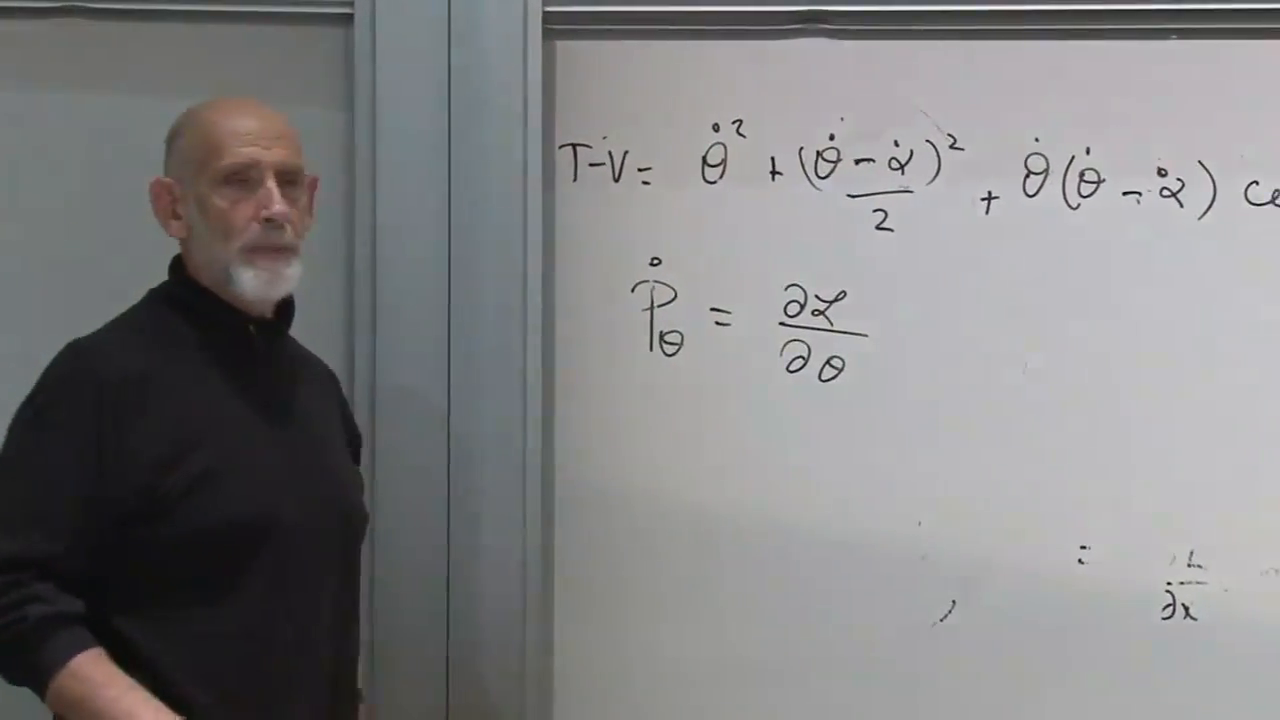
\includegraphics[width=0.84\textwidth]{lecture_06_figure_02.png}
  \caption{無重力時的擺系統計算，以及\(\dot p_\theta=\partial L/\partial\theta\)。上方黑板行列出的是問題中提到、符號不一致的局部記號；整理後的公式見式~\eqref{eq:l6-double-kinetic}。}
  \lectureframe{00:45:50}
\end{figure}

知道\(T\)與\(V\)後，其餘方程便可透過微分求得。桿的張力以及維持桿長固定的力，再次因座標的選擇而不必明確處理。

\subsection{守恆的意義與限度}

\begin{classroomqa}
  \audiencequestion{能否直接從方程看出雙擺是否具有混沌行為？
  \lecturetimestamp{00:44:57--00:45:25}}
  \lecturerresponse{通常無法只靠簡單觀察判斷。系統可能隨著參數或能量的變化，從規則運動轉為混沌運動。要探討這個問題，需要比方程表面形式更完整的架構，後面會再談到。}
\end{classroomqa}

\begin{classroomqa}
  \audiencequestion{在保守系統中，每個\(\dot p_i\)都等於零嗎？
  \lecturetimestamp{00:45:25--00:46:24}}
  \lecturerresponse{不一定。一般方程是
  \(\dot p_i=\partial L/\partial q_i\)。只有當\(q_i\)是循環座標時，它才會為零。循環座標是特別簡單的情況：透過對稱變換使一個座標平移，同時其他座標保持不變。}
\end{classroomqa}

如果唯一的目標是進行數值演化，即使座標系不方便，也仍然可行；只是方程會更長。巧妙選擇座標的好處在於概念上的清晰：還沒解方程，就已經能看出哪個動量守恆。

\begin{classroomqa}
  \audiencequestion{沒有重力時，雙擺的運動會像單一自由擺那樣簡單嗎？
  \lecturetimestamp{00:47:02--00:47:35}}
  \lecturerresponse{單一自由轉子會等角速度轉動，因為它的角動量決定了運動。雙擺即使保持總角動量守恆，相對運動仍可能十分複雜。若兩個角速度初始都為零，系統便保持靜止；否則兩部分會相互作用。}
\end{classroomqa}

\begin{classroomqa}
  \audiencequestion{沒有重力時，\(\dot\theta\)與\(\dot\alpha\)各自會保持不變嗎？
  \lecturetimestamp{00:47:36--00:52:42}}
  \lecturerresponse{不會。守恆表示\(\dot p_\theta=0\)，而不是\(\ddot\theta=0\)或\(\ddot\alpha=0\)。\(p_\theta=\partial L/\partial\dot\theta\)的表式包含兩個角速度，且取決於\(\alpha\)。桿會傳遞力矩，使兩個擺錘得以交換角動量與能量。這類似以彈簧連接的兩個質點：總動量與質心速度保持不變，但各質點的速度會振盪。對應的轉動量是某個特定的集體組合，而不是任一角度本身。}
\end{classroomqa}

\begin{classroomqa}
  \audiencequestion{交換角動量的力是透過桿傳遞的嗎？
  \lecturetimestamp{00:52:43--00:53:34}}
  \lecturerresponse{是。沿桿傳遞的力不一定通過另一個運動所繞的支點，因此可能對該支點產生力矩。力矩就是力使物體轉動的效應；在這裡，它造成各自非零的角加速度。}
\end{classroomqa}

\section{作為第三種力學表述的哈密頓量}

哈密頓量就是能量，但這只是它的第一層意義。它也是第三種力學表述的基礎。牛頓方程以力和加速度描述運動；駐作用量原理則導出尤拉--拉格朗日方程。對於正則系統，哈密頓力學與後者等價，但使用的變數與幾何觀點不同。

改用\(q_i\)與其共軛動量\(p_i\)，而不使用\(q_i\)和\(\dot q_i\)。具有\(n\)個自由度的系統，無論採用哪種描述，都需要\(2n\)個數來表示狀態：可以是位置與速度，也可以是位置與動量。兩者之間的連結是
\begin{equation}
  p_i=\frac{\partial L}{\partial\dot q_i}.
  \label{eq:l6-legendre-map}
\end{equation}
若這些關係可以反解出速度\(\dot q_i(q,p)\)，便定義
\begin{equation}
  H(q,p)=\sum_i p_i\dot q_i-L(q,\dot q).
  \label{eq:l6-hamiltonian-definition}
\end{equation}
如此一來，右側的速度便可消去，改以\(q\)和\(p\)表示。這種可逆性就是正則勒讓德變換所需的假設。奇異拉格朗日量則需要更一般的約束理論；這種初等構造不適用於它們。

\subsection{微積分之前先談可逆性}

回想一組以箭頭連結的有限個抽象狀態。若兩個較早的狀態都演變到同一個較晚的狀態，確定性規則仍可能不可逆：未來是唯一的，過去卻不唯一。若將所有箭頭反向，則會出現相反的問題：一個狀態分岔出多個未來。前一種圖中箭頭匯聚，後一種圖中箭頭發散。

\begin{figure}[htbp]
  \centering
  \includegraphics[width=0.86\textwidth]{lecture_06_figure_11.png}
  \caption{用來對照可逆循環，以及不允許的匯聚與發散之抽象狀態映射。}
  \lectureframe{00:56:20}
\end{figure}

哈密頓流將為這個說法提供連續版本。相空間中的一團點可以移動、變形，但不會形成消除狀態差異的匯，也不會形成從單一狀態產生多個未來的源。證明留待後續；目前先由這些圖示引出幾何觀點。

\begin{classroomqa}
  \audiencequestion{這張抽象狀態圖是否應解讀為物體在重力場中運動？
  \lecturetimestamp{00:58:02--00:58:35}}
  \lecturerresponse{不是。圖中的點只是抽象狀態，箭頭則表示狀態變化的規則。這張圖沒有任何空間或重力上的意義。}
\end{classroomqa}

\begin{classroomqa}
  \audiencequestion{要如何區分不允許的收斂狀態映射與黑洞？
  \lecturetimestamp{00:58:40--00:59:28}}
  \lecturerresponse{這需要非常細緻的分析。這個問題問得合理，但要正確回答，必須仔細描述完整狀態及其量子引力演化。單靠這張簡單圖示不足以判定。}
\end{classroomqa}

\section{適合相空間描述的振子}

在推導一般方程之前，先考慮一個刻意採用適合相空間變數來表示的諧振子：
\begin{equation}
  L=\frac{1}{2\omega}\dot q^2-\frac{\omega}{2}q^2.
  \label{eq:l6-rescaled-lagrangian}
\end{equation}
其共軛動量為
\begin{equation}
  p=\frac{\partial L}{\partial\dot q}=\frac{\dot q}{\omega},
  \qquad
  \dot q=\omega p.
  \label{eq:l6-rescaled-momentum}
\end{equation}
代入式~\eqref{eq:l6-hamiltonian-definition}，可得
\begin{align}
  H&=p\dot q-L\\
   &=\omega p^2-\frac{\omega p^2}{2}+\frac{\omega q^2}{2}
    =\frac{\omega}{2}(p^2+q^2).
  \label{eq:l6-oscillator-hamiltonian}
\end{align}

\begin{figure}[htbp]
  \centering
  \includegraphics[width=0.86\textwidth]{lecture_06_figure_12.png}
  \caption{適配振子的勒讓德變換，以及對稱形式的哈密頓量\(H=\tfrac{\omega}{2}(p^2+q^2)\)。}
  \lectureframe{01:08:20}
\end{figure}

\(q\)與\(p\)構成的空間就是相空間。一個自由度對應二維平面；兩個自由度則對應四維相空間。振子能量固定時，
\begin{equation}
  p^2+q^2=\frac{2H}{\omega},
  \label{eq:l6-energy-circle}
\end{equation}
所以軌跡會保持在圓上。能量守恆將運動限制在其中一條曲線上。

\begin{figure}[htbp]
  \centering
  \includegraphics[width=0.82\textwidth]{lecture_06_figure_13.png}
  \caption{振子相平面中的巢狀等能圓；\(q\)為水平軸，\(p\)為垂直軸。}
  \lectureframe{01:13:20}
\end{figure}

\section{推導哈密頓方程}

這項推導是多變數函數微分的練習。對於\(F(q,p)\)，
\begin{equation}
  \delta F=\sum_i\left(
  \frac{\partial F}{\partial q_i}\delta q_i
  +\frac{\partial F}{\partial p_i}\delta p_i\right).
  \label{eq:l6-total-differential}
\end{equation}
從不同方向都能讀出係數：\(\delta q_i\)的係數是\(\partial F/\partial q_i\)，而\(\delta p_i\)的係數是\(\partial F/\partial p_i\)。

現在對\(H\)的定義式取變分：
\begin{align}
  \delta H
  &=\sum_i\left(\dot q_i\,\delta p_i
       +p_i\,\delta\dot q_i\right)-\delta L\\
  &=\sum_i\left(\dot q_i\,\delta p_i
       +p_i\,\delta\dot q_i
       -\frac{\partial L}{\partial q_i}\delta q_i
       -\frac{\partial L}{\partial\dot q_i}\delta\dot q_i\right).
  \label{eq:l6-vary-hamiltonian}
\end{align}
由於\(\partial L/\partial\dot q_i=p_i\)，兩個\(\delta\dot q_i\)項會相消。尤拉--拉格朗日方程給出\(\partial L/\partial q_i=\dot p_i\)，剩下
\begin{equation}
  \delta H=\sum_i\left(\dot q_i\,\delta p_i
                     -\dot p_i\,\delta q_i\right).
  \label{eq:l6-reduced-variation}
\end{equation}

\begin{figure}[htbp]
  \centering
  \includegraphics[width=0.86\textwidth]{lecture_06_figure_14.png}
  \caption{\(\delta H\)依乘積法則展開後、\(p_i\,\delta\dot q_i\)項相消之前的形式。}
  \lectureframe{01:18:40}
\end{figure}

比較式~\eqref{eq:l6-reduced-variation}與式~\eqref{eq:l6-total-differential}的一般微分式，對照獨立係數即可得到哈密頓方程：
\begin{equation}
  \boxed{
  \dot q_i=\frac{\partial H}{\partial p_i},
  \qquad
  \dot p_i=-\frac{\partial H}{\partial q_i}.}
  \label{eq:l6-hamilton-equations}
\end{equation}

\begin{figure}[htbp]
  \centering
  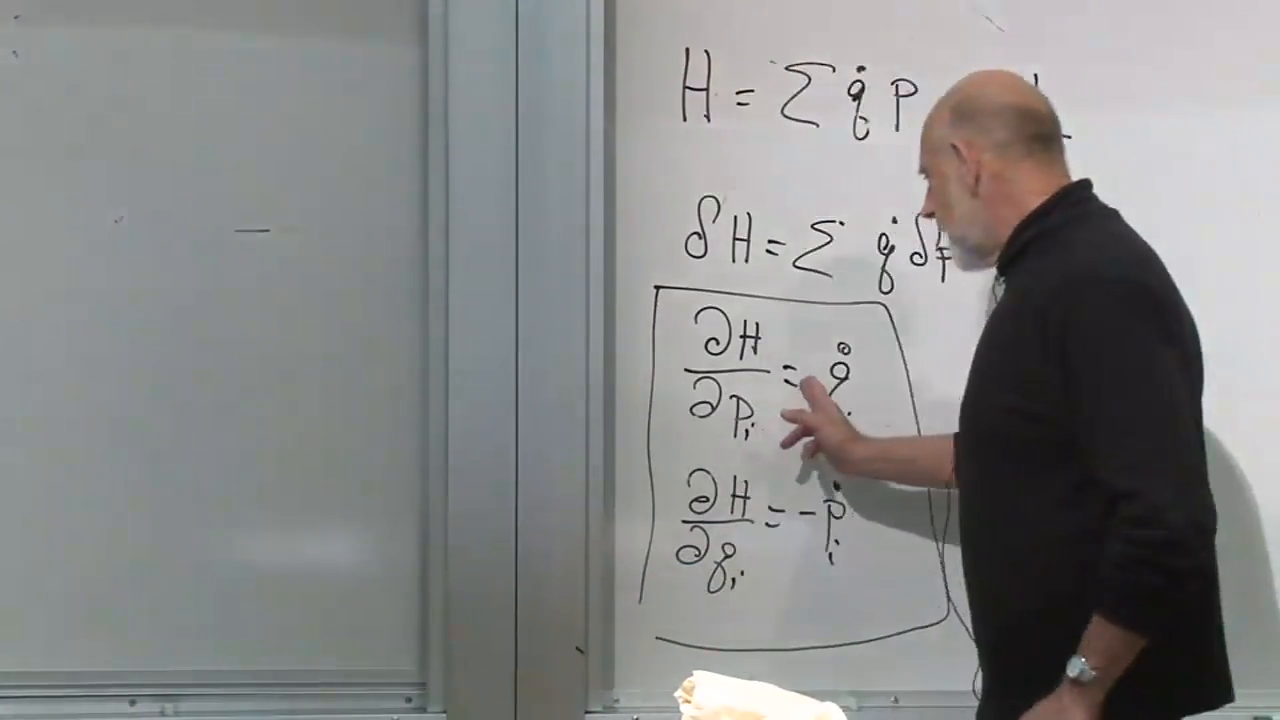
\includegraphics[width=0.78\textwidth]{lecture_06_figure_03.png}
  \caption{哈密頓量的定義、其變分，以及框列的正則方程。}
  \lectureframe{01:22:18}
\end{figure}

對\(n\)個座標而言，這是\(2n\)個一階方程。尤拉--拉格朗日表述則提供\(n\)個二階方程。兩種表述所需的初始資料數量相同，物理內容也完全相同。

\section{振子運動就是剛性旋轉}

將式~\eqref{eq:l6-hamilton-equations}套用於式~\eqref{eq:l6-oscillator-hamiltonian}，可得
\begin{equation}
  \dot q=\omega p,
  \qquad
  \dot p=-\omega q.
  \label{eq:l6-oscillator-first-order}
\end{equation}
對第一個方程微分，再利用第二個方程，得到
\begin{equation}
  \ddot q=\omega\dot p=-\omega^2q.
  \label{eq:l6-oscillator-second-order}
\end{equation}
因此，這兩個一階方程恰好等同於通常的二階振子方程，並包含動量的定義。

在相空間中，\((q,p)\)處的速度向量為\((\dot q,\dot p)=(\omega p,-\omega q)\)，與等能圓相切。每條半徑都以相同的角速度\(\omega\)旋轉。整個平面可以想成剛性的風車，也可以想成不可壓縮的虛構流體。平面上的點會循環流動，不會擠入某個匯，也不會從某個源向外發散。

\begin{figure}[htbp]
  \centering
  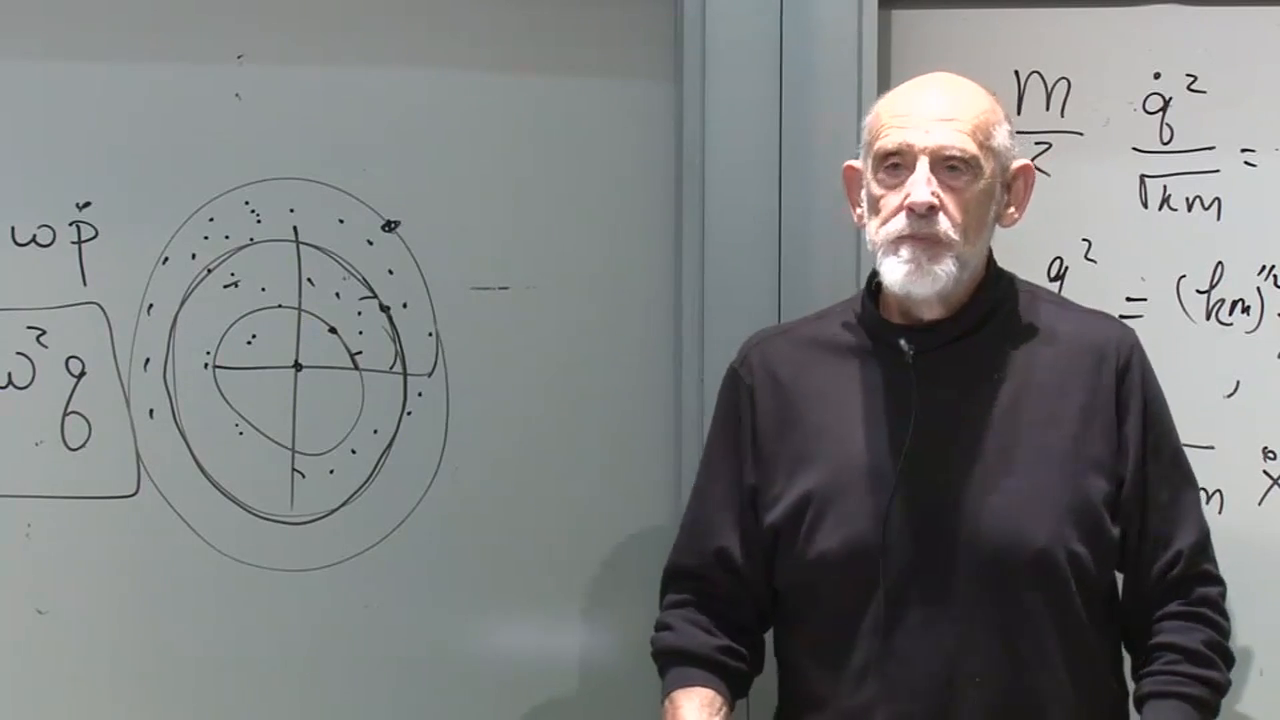
\includegraphics[width=0.86\textwidth]{lecture_06_figure_04.png}
  \caption{一團初始點分布在巢狀的相空間軌跡上。哈密頓演化會帶動這團點，而不會使它塌縮到某個偏好的狀態。}
  \lectureframe{01:39:27}
\end{figure}

\begin{figure}[htbp]
  \centering
  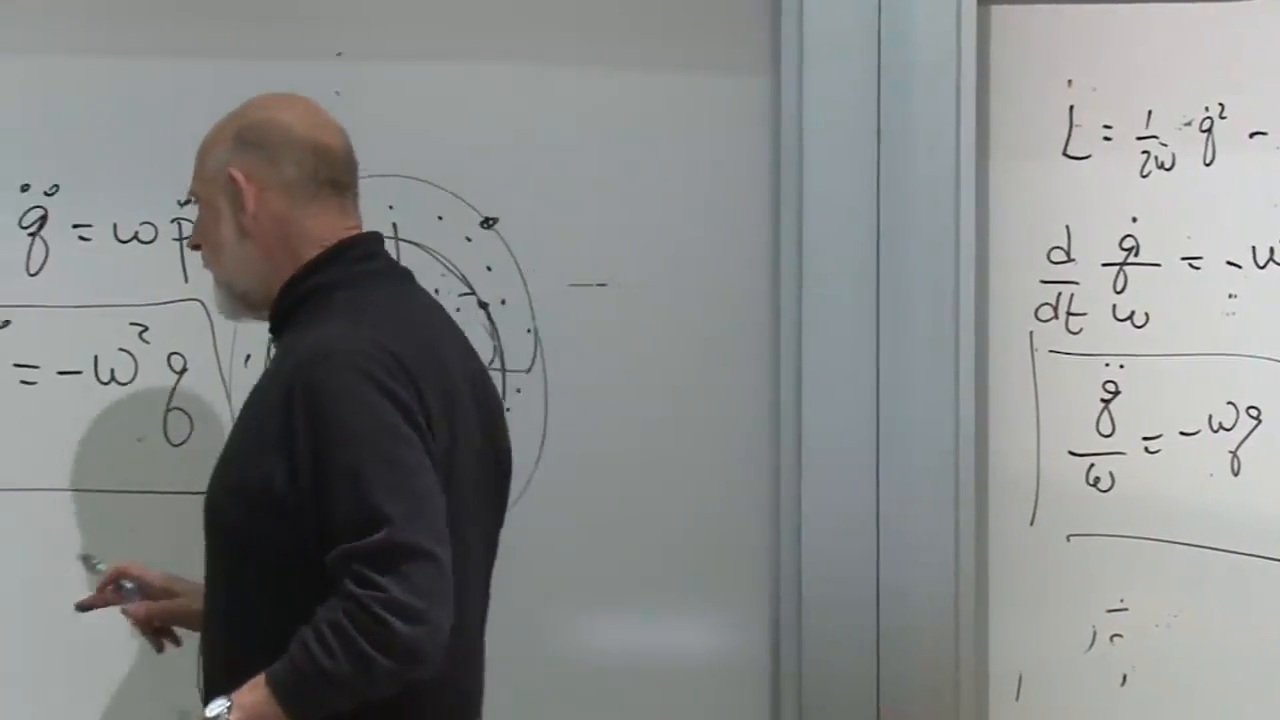
\includegraphics[width=0.90\textwidth]{lecture_06_figure_05.png}
  \caption{振子相圖，旁列等價的尤拉--拉格朗日方程\(\ddot q/\omega=-\omega q\)。}
  \lectureframe{01:42:10}
\end{figure}

下一步會將流體類比嚴格化為定理：哈密頓流在局部不會收斂或發散。這個結果會把連續力學與課程開頭討論的可逆狀態映射重新連結起來。

\section{從座標選擇引出的問題}

\begin{classroomqa}
  \audiencequestion{速度可以用\(q\)和\(p\)求解，這項假設究竟是定理，還是物理系統的經驗性質？
  \lecturetimestamp{01:29:08--01:29:45}}
  \lecturerresponse{在這套初等推導中，這是一項經驗規律，其更深層的動機來自量子力學。更精確地說，式~\eqref{eq:l6-legendre-map}對速度的雅可比矩陣必須非奇異。現代力學也包含重要的奇異拉格朗日量，尤其是受約束系統與規範系統；但其哈密頓表述需要額外的約束處理架構。}
\end{classroomqa}

對量綱的疑問可以說明，為什麼振子會寫成式~\eqref{eq:l6-rescaled-lagrangian}中不熟悉的形式。先從一般座標\(x\)出發：
\begin{equation}
  L=\frac{m}{2}\dot x^2-\frac{k}{2}x^2,
  \qquad
  \omega=\sqrt{\frac{k}{m}}.
  \label{eq:l6-ordinary-oscillator}
\end{equation}
令
\begin{equation}
  q=(km)^{1/4}x.
  \label{eq:l6-oscillator-rescaling}
\end{equation}
於是\(q^2=\sqrt{km}\,x^2\)且\(\dot q^2=\sqrt{km}\,\dot x^2\)，式~\eqref{eq:l6-ordinary-oscillator}便恰好轉換為式~\eqref{eq:l6-rescaled-lagrangian}。新的\(q\)是經過調整的廣義座標，不是長度；它的共軛動量\(p\)也不是一般的力學動量\(p_x=m\dot x\)。

\begin{figure}[htbp]
  \centering
  \includegraphics[width=0.86\textwidth]{lecture_06_figure_15.png}
  \caption{從一般振子座標\(x\)到調整後座標\(q=(km)^{1/4}x\)的量綱重標度。}
  \lectureframe{01:36:10}
\end{figure}

\begin{classroomqa}
  \audiencequestion{\(\omega p=\dot q\)如何符合量綱一致性？為什麼要選用這些變數？
  \lecturetimestamp{01:29:46--01:39:22}}
  \lecturerresponse{符號\(q\)不必具有長度量綱，其共軛動量\(p\)也不必具有\(m\dot x\)的量綱。式~\eqref{eq:l6-oscillator-rescaling}中的重標度保留了拉格朗日量的量綱，並使\(q\)與\(p\)對稱地出現在\(H\)中。在原來的變數中，
  \[
    H=\frac{p_x^2}{2m}+\frac{kx^2}{2},
  \]
  因此，\((x,p_x)\)平面上的等能曲線是橢圓；在調整後的\((q,p)\)平面上則是圓。選用這種重標度，就是為了凸顯這項對稱性。}
\end{classroomqa}

\begin{classroomqa}
  \audiencequestion{\(2n\)個一階哈密頓方程，怎麼會等價於\(n\)個二階拉格朗日方程？
  \lecturetimestamp{01:39:24--01:42:30}}
  \lecturerresponse{對振子而言，將\(\dot q=\omega p\)微分並代入\(\dot p=-\omega q\)，這一對方程便化為\(\ddot q=-\omega^2q\)。若直接從拉格朗日量出發，則得到
  \[
    \frac{d}{dt}\left(\frac{\dot q}{\omega}\right)
      =-\omega q,
  \]
這是相同的二階方程。一個哈密頓方程可視為以速度定義動量，另一個則描述該動量如何演化。}
\end{classroomqa}

\section{相空間與位能為何重要}

\begin{classroomqa}
  \audiencequestion{哈密頓量的強大作用，是否表示相空間在幾何表述上優於位形空間？
  \lecturetimestamp{01:42:33--01:44:38}}
  \lecturerresponse{兩者用途不同。相空間能格外清楚地呈現循環、等能面，以及沒有收斂或發散的特性；位形空間則可能更適合探討其他問題。重視\(H\)更深層的原因在於，它在量子力學中會成為核心且更直觀的對象，而量子力學正是這套力學所引向的現代學科之一。}
\end{classroomqa}

\begin{classroomqa}
  \audiencequestion{勢能應視為力的積分嗎？
  \lecturetimestamp{01:44:40--01:45:45}}
  \lecturerresponse{對保守力而言，這種說法成立，但須相差一個常數，且符號要適當。更實用的做法是將勢能視為基本量，再由它導出廣義力：
  \[
    F_i=-\frac{\partial V}{\partial q_i}.
  \]
當\(L=T-V\)且動能不明確依賴\(q_i\)時，這正是\(\dot p_i=\partial L/\partial q_i\)中出現的那一項。}
\end{classroomqa}

\begin{classroomqa}
  \audiencequestion{這條邁向現代物理的路徑，旨在闡明哪些前沿問題？
  \lecturetimestamp{01:45:46--01:47:47}}
  \lecturerresponse{這條路徑通往量子引力與宇宙學、基本粒子物理（包括希格斯部門與中微子）、相對論、弦論及量子場論。持續存在的理論難題，是如何將這些領域整合成一個連貫架構，尤其是如何結合量子力學與引力，以及宇宙學與粒子物理。這是在陳述2011年當時的前沿狀況，並非宣稱問題當時已經解決。}
\end{classroomqa}

這兩個受約束系統的例子與振子，如今可納入同一幅圖景。廣義座標排除了不必要的力；對稱性則選出守恆的正則動量。勒讓德變換以動量取代速度，而哈密頓方程將動力學描述為相空間中的流。對振子而言，這個流是剛性旋轉；對一般系統而言，其幾何結構將賦予可逆運動明確的連續意義。